\documentclass[11pt,letterpaper,final]{report}
\usepackage[utf8]{inputenc}
\usepackage[francais]{babel}
\usepackage[T1]{fontenc}
\usepackage{amsmath}
\usepackage{amsfonts}
\usepackage{amssymb}
\usepackage{graphicx}
\usepackage{lmodern}
\usepackage[left=2.54cm,right=2.54cm,top=2.54cm,bottom=2.54cm]{geometry}
\begin{document}
\chapter{Cross validation entre les différentes plateformes de simulations}
\section{Pont DCP/DCN: Validation PSIM/SPS}

Les résultats de la simulation du pont DCP/DCN sur les électroaimants, contenant la référence de courant et le courant réel ainsi que la tension appliquée et moyenne sont présentés à la figure \ref{figDCPDCN1}. Les résultats de simulation correspondant implantés dans une simulation sur le logiciel PSIM sont présentés à la figure \ref{figDCPDCN2}.
\begin{figure}[htb]
\centering
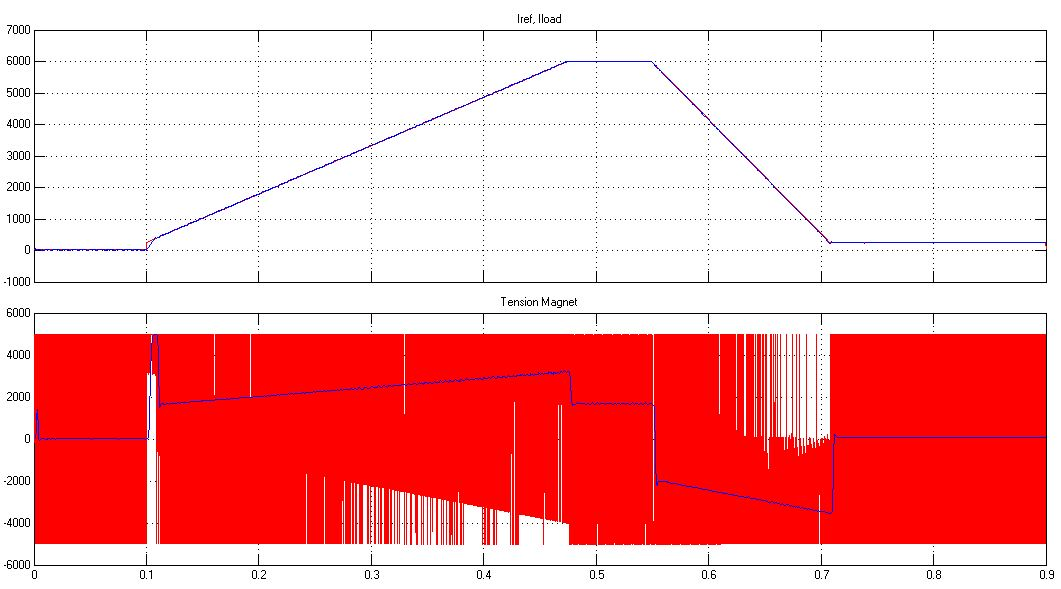
\includegraphics[scale=0.4]{fig/resul_sim.jpg}
\caption{Courant de référence par rapport au courant réel, tension appliquée et moyenne appliqués sur les électroaimants au moyen d'une simulation sur SPS}
\label{figDCPDCN1}
\end{figure}
\begin{figure}[htb]
\centering
\includegraphics[scale=0.6]{fig/resul_PSIM.jpg}
\caption{Courant de référence par rapport au courant réel, tension appliquée et moyenne appliqués sur les électroaimants au moyen d'une simulation sur PSIM}
\label{figDCPDCN2}
\end{figure}


\subsection{Calcul de la tension moyenne}

La fonction "Mean" de SPS et celle correspondant sur PSIM ne donne pas exactement le même résultat de simulation. Pour le montrer, chacune des fonctions sur les 2 simulateurs a été testée avec un signal sinusoïdal de  100V d'amplitude crête avec un niveau CC de 50V moyen et à une fréquence de 1KHz. Les figures \ref{dis_mean} et \ref{D_mean} montrent les résulats obtenus avec une fréquence de 500Hz du moyenneur.



\begin{figure}[h]
\centering
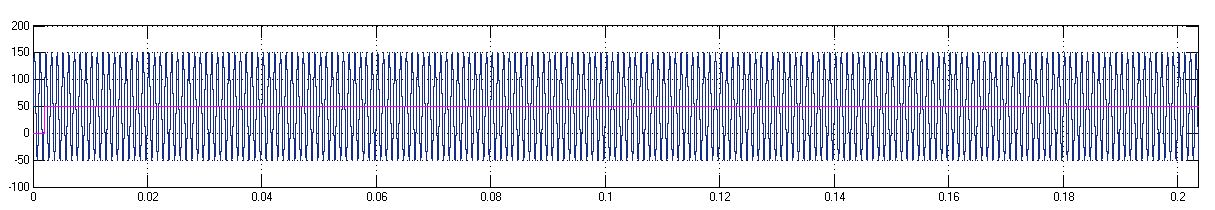
\includegraphics[scale=0.5]{fig/moy_sim.jpg}
\caption{Réponse de la fonction "Discrete Mean" pour un signal sinusoïdal de 1kHz 100V crête avec un niveau CC de 50V sur SPS}
\label{dis_mean}
\end{figure}

\begin{figure}[h]
\centering
\includegraphics[scale=0.5]{fig/moy_PSIM.jpg}
\caption{Réponse du bloc "DC Voltmeter" pour un signal sinusoïdal de 1kHz 100V crête avec un niveau CC de 50V sur PSIM}
\label{D_mean}
\end{figure}


\begin{figure}[ht]
\centering
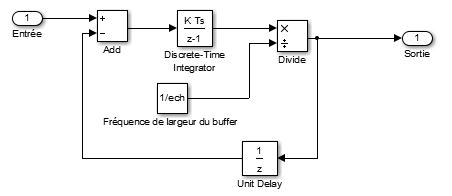
\includegraphics[scale=0.8]{fig/moy.jpg}
\caption{Fonction de moyennage de la tension}
\label{moy}
\end{figure}
On remarque bien que les résultats sont différents dans les figures \ref{dis_mean} et \ref{D_mean}. La tension moyenne calculé sur SPS est plus précise et varie moins que celle de PSIM. La précision est telle que le résultat de PSIM est variant sur chaque période tandis que celle de SPS a une apparence droite. Par contre, le temps de réponse de SPS est plus long que celui de PSIM. Par conséquent, une fonction de moyennage personnalisée a été développée dans les 2 simulateurs pour avoir un fonctionnement identique. La figure \ref{moy} représente la fonction qui est constituée d'un intégrateur avec un gain unitaire. Cette valeur est passée dans un gain de 3000 qui contrôle la sensibilité du calcul de moyennage. De plus, 10 fonctions de moyennage ont été cascadées pour optimiser le résultat et avoir une moyenne avec une oscillation négligeable. Comme les filtres donnent le même résultat sur les deux plateformes donc le fonctionnement de la fonction de moyennage sur PSIM est identique et donne le même résultat que celle de SPS si le signal d'entrée est le même. La figure~\ref{rep_freq_mo} montre la réponse en fréquence du moyenneur. Étant donné que la tenion à charge est supposé avoir une fréquence de 1000Hz, on déduit que le calcul de la tension moyenne est très précise.



\begin{figure}[h!]
\centering
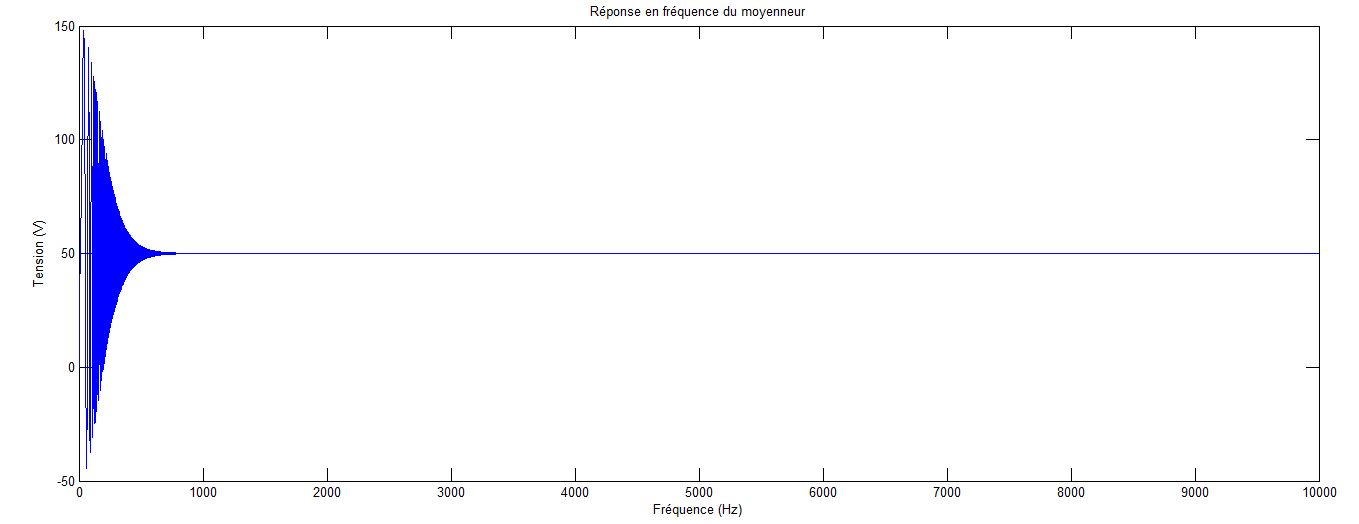
\includegraphics[scale=0.4]{fig/rep_freq_moy.jpg}
\caption{Réponse en fréquence de la fonction permettant le calcul de la tension moyenne}
\label{rep_freq_mo}
\end{figure}

\begin{figure}[h!]
\centering
\includegraphics[scale=0.4]{fig/tmoyPSIM_sim.jpg}
\caption{Courbes de tension moyenne aux bornes de l'électroaimant superposées pour les simulateurs PSIM et SPS}
\label{moyt}
\end{figure}
\begin{figure}[h!]
\centering
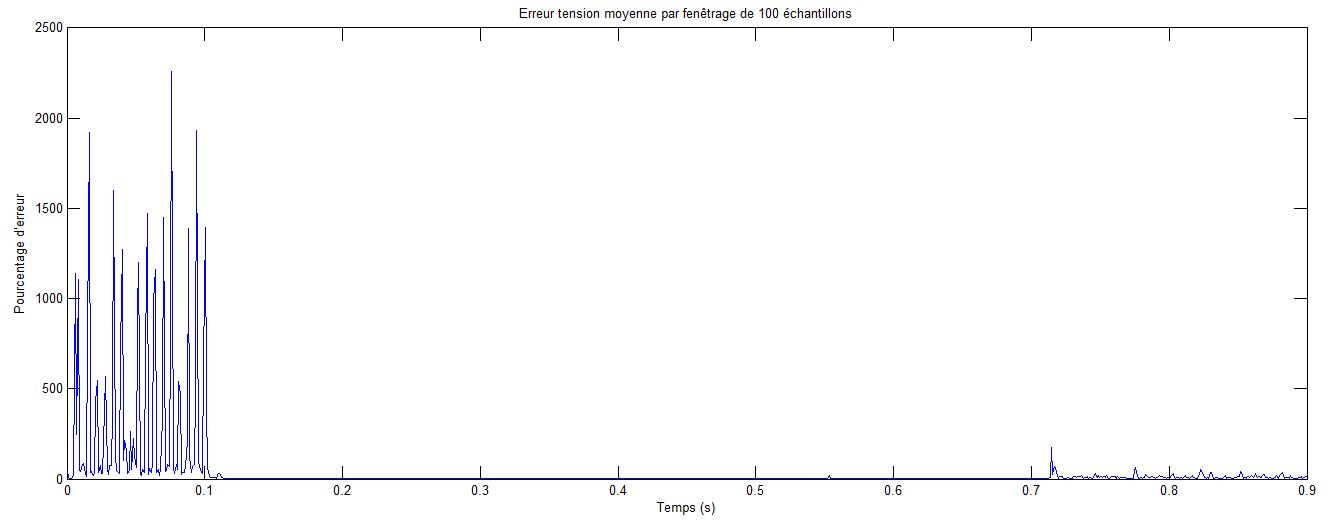
\includegraphics[scale=0.4]{fig/erre_ten_fen.jpg}
\caption{Courbe représentant l'erreur de la tension moyenne entre SPS et PSIM en pourcentage avec un fenêtrage de 100 échantillons}
\label{err_ten}
\end{figure}
\begin{figure}[h!]
\centering
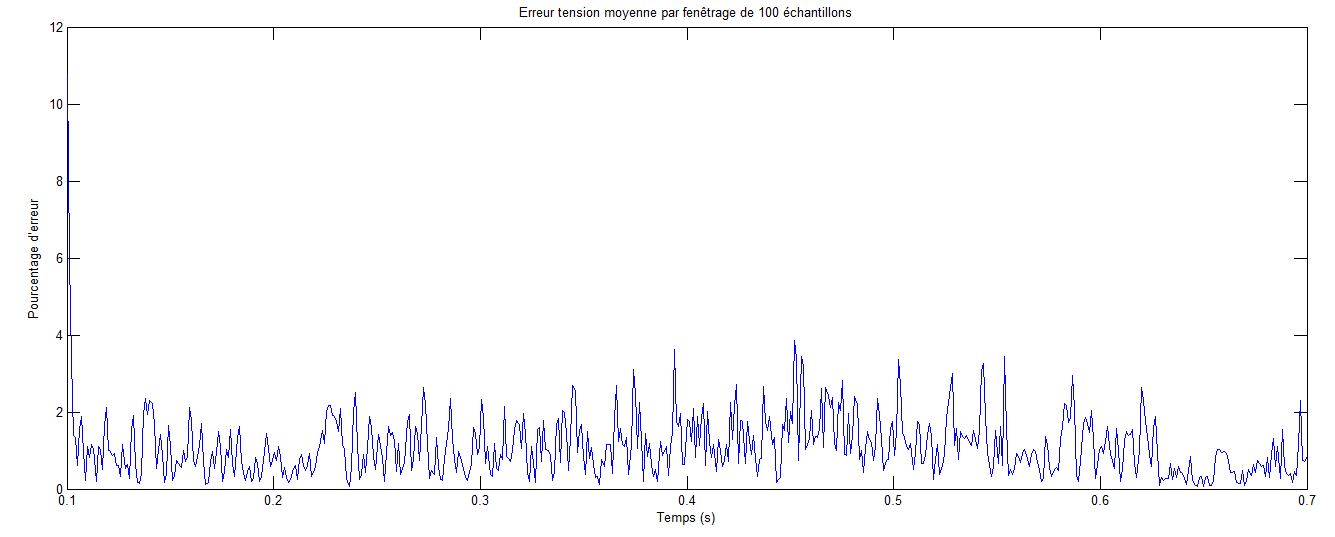
\includegraphics[scale=0.4]{fig/err_ten_imp.jpg}
\caption{Courbe représentant l'erreur de la tension moyenne entre SPS et PSIM en pourcentage avec un fenêtrage de 100 échantillons entre 0.1 et 0.7 secondes}
\label{err_ten_imp}
\end{figure}
Sur la figure \ref{moyt} on capte la différence relative entre la tension moyenne sur PSIM et SPS. La courbe en vert représente la réponse sur PSIM et en bleu celle sur SPS. La différence observé est dû au fait que sur SPS nous utilisons des IGBT idéaux donc qui commutent instantanément, tandis que sur PSIM ce sont des IGBT qui ont un temps de commutation faible mais non négligeable. Leur modélisation présente une différence non négligeable. De sorte que, c'est normal qu'on n'ait pas le même résultat car la simulation de PSIM a une perte de commutation tandis que celle de SPS n'en a pas. Il faut aussi prendre en compte que l'algorithme de PSIM et SPS n'est pas la même au niveau des passage à zéros ce qui procure une différence de fonctionnement entre les simulateurs. Par contre, on constate que les résultats sont très semblables même si l'erreur moyenne est de 41.4868\%, elle est calculée selon l'équation \ref{eq1}. Étant donnée que l'erreur varie en fonction du niveau de la tension moyenne, la figure~\ref{err_ten} montre l'erreur de la tension moyenne avec un fenêtrage de 100 échantillons. Ça représente l'erreur en différents points de fonctionnement. On observe bien que lorsque l'impulsion de courant est produite, l'erreur de tension moyenne devient très faible entre les deux simulateurs. En somme, il est possible de confirmer la concordance des résultats de la simulation du pont DCP/DCN sur les 2 simulateurs. Il faut aussi comprendre que les IGBT de SPS sont plus dévéloppés que ceux de PSIM. Ils contiennent un snubber RC intégré, ce qui n'est pas le cas sur PSIM. De plus, sur SPS il est possible de mettre la valeur d'un condensateur à inf ce qui représente pour le snubber un fonctionnement purement résistif. PSIM ne permet pas de mettre un condensateur à inf, il faut le mettre plutôt à 0 si on veut que le condensateur ne soit pas tenu en compte.


\begin{equation}
Erreur = \frac{\frac{1}{T}\int_TV_{moy SPS}(t)dt-\frac{1}{T}\int_TV_{moy PSIM}(t)dt}{\frac{1}{T}\int_TV_{moy SPS}(t)dt}
\label{eq1}
\end{equation}




\subsection{Calcul du courant}
Les résultats sur les deux plateformes, concernant la différence obtenus au niveau du courant dans les électroaimants, ont été comparés. La différence obtenue est de 5.8615\% entre PSIM et SPS en utilisant la valeur moyenne de l'erreur entre PSIM et SPS, suivant l'équation \ref{eq2}. La simulation de PSIM valide la simulation sur SPS puisque les 2 simulations fournissent des résultats analogues présentant une faible différence en dessous du seuil de 10\% comme on peu le voir sur la figure de courant~\ref{comp_PSIM_SPS}. La figure~\ref{err_cou} permet de bien confirmer la concordance des deux simulateurs au niveau ou l'impulsion de courant est crée ce qui assure d'avoir une bonne précision au niveau des spectres attendus par rapport à l'impulsion de courant.


\begin{equation}
Erreur = \frac{\frac{1}{T}\int_T I_{SPS}(t)dt-\frac{1}{T}\int_T I_{PSIM}(t)dt}{\frac{1}{T}\int_T I_{SPS}(t)dt}
\label{eq2}
\end{equation}


\begin{figure}[ht]
\centering
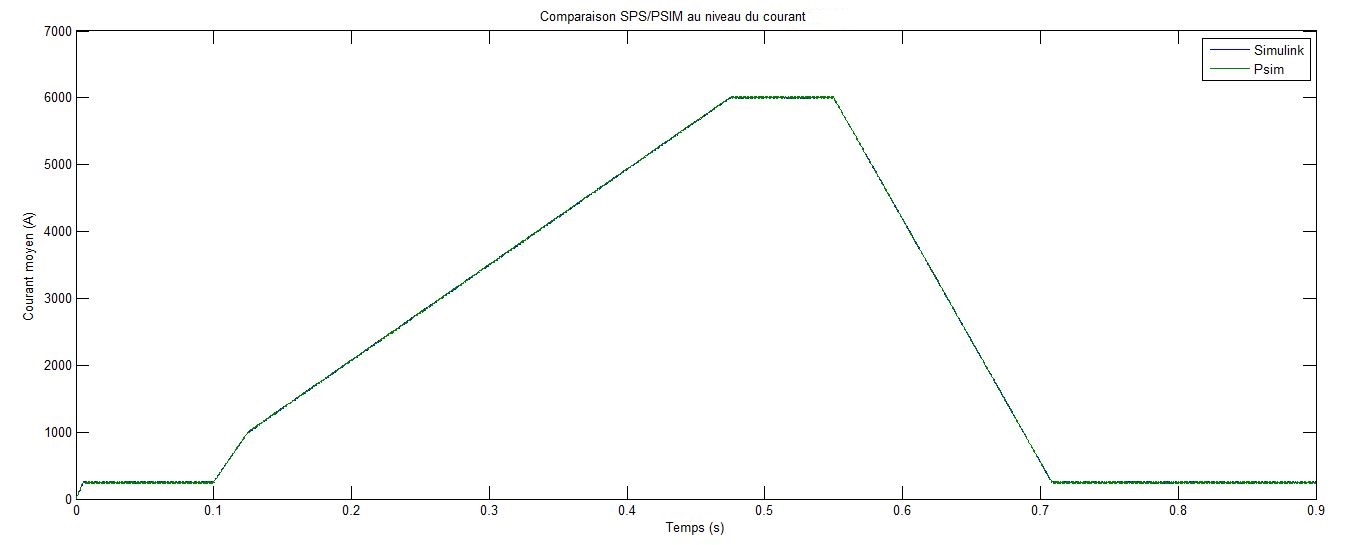
\includegraphics[scale=0.5]{comp_PSIM_SPS.jpg}
\caption{Le courant sur la charge PSIM et SPS}
\label{comp_PSIM_SPS}
\end{figure}


\begin{figure}[ht]
\centering
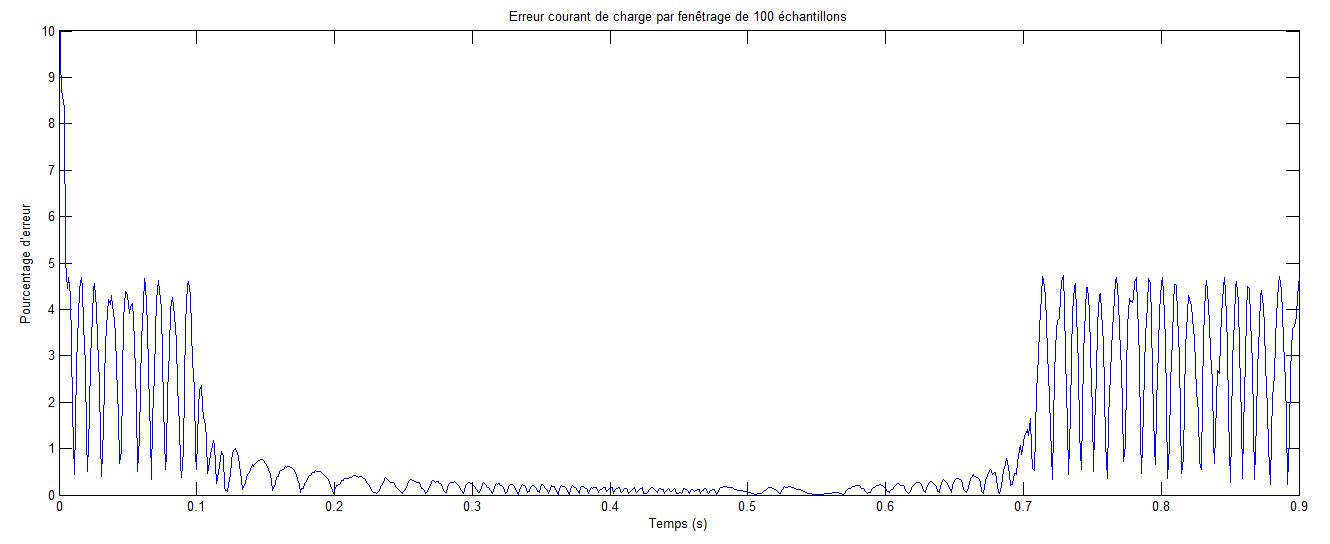
\includegraphics[scale=0.5]{fig/err_cour_fen.jpg}
\caption{Erreur du courant avec un fenêtrage de 100 échantillons}
\label{err_cou}
\end{figure}

\end{document}